\documentclass[a4paper]{article}

\usepackage[english]{babel}
\usepackage[utf8x]{inputenc}
\usepackage{amsmath}
\usepackage{graphicx}
\usepackage[colorinlistoftodos]{todonotes}

\title{Computation of the five-bar mechanism models}
\author{Damien SIX}
\date{August 3, 2021}

\begin{document}
\maketitle
\section{Introduction}
This document details the equations of the kinematic and dynamic models of a five-bar mechanism. This recall of the AMORO course is provided to help the students in performing the AMORO lab.

The kinematic architecture of the five-bar mechanism is shown in Fig.\ref{fig:5bar}. In the context of the AMORO lab, the geometric parameters are: 
\begin{itemize}
\item    Bar length (all bars are equal length): $l$ = 0.09 m 
\item    Distance between the two active joints: $d=d_{A_{11}A_{21}}$ = 0.118 m 
\end{itemize}
    
\begin{figure}[h!]
\centering
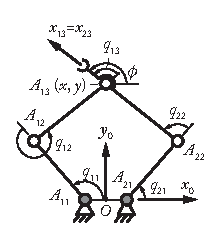
\includegraphics[width=0.6\textwidth]{RuRRRRu_kin.eps}
\caption{Kinematic architecture of the five-bar mechanism. Joints located at A11 and A21 are actuated.}
\label{fig:5bar}
\end{figure}

\section{Geometric models}
%
\subsection{Direct geometric model}
\begin{figure}[h!]
\centering
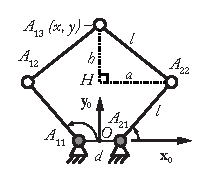
\includegraphics[width=0.6\textwidth]{DGM5bar.eps}
\caption{Kinematic architecture of the five-bar mechanism}
\label{fig:DGM}
\end{figure}
The direct geometric model gives the position of the end-effector $(x, y)$ as a function of the active joints coordinates $(q_{11}, q_{21})$ and the assembly mode.

Using Figure \ref{fig:DGM}, the direct geometric model can be computed according to the following method. First, the vector $\overrightarrow{A_{22}H}$ is computed.
\begin{equation}
    \begin{aligned}
        \overrightarrow{A_{22}H} &= \frac{1}{2} \overrightarrow{A_{22}A_{12}}\\
        &= \frac{1}{2} (-\overrightarrow{A_{21}A_{22}} + \overrightarrow{A_{21}A_{11}} +\overrightarrow{A_{11}A_{12}})\\
        &= \frac{1}{2}\begin{bmatrix}
        -l\cos{q_{21}}-d+l\cos{q_{11}}\\
        -l\sin{q_{21}}+l\sin{q_{11}}
        \end{bmatrix}
    \end{aligned}
\end{equation}
There are two solutions for the point $A_{13}$, relative to the two assembly mode of the robot. They are obtained by the 90° rotation (clockwise and counter-clockwise) of the vector $\overrightarrow{A_{22}H}$ scaled to the length $h$ (see \ref{fig:DGM}), giving
%
\begin{equation}
\overrightarrow{HA_{13}}=\gamma\frac{h}{a}\begin{bmatrix}
0&-1\\1&0
\end{bmatrix}\overrightarrow{A_{22}H}
\end{equation}
%
with $a = d_{A_{22}H}$ and $h = \sqrt{l²-a²}$.\\
$\gamma$ takes two values, +1 and -1, depending of the direction of \textit{assembly mode}. Each value of $\gamma$ correspond to one assembly mode.

The position of the end-effector is then given by
\begin{equation}
    \overrightarrow{OA_{13}}=\overrightarrow{OA_{21}}+\overrightarrow{A_{21}A_{22}}+\overrightarrow{A_{22}H}+\overrightarrow{HA_{13}}
\end{equation}
%%%%%%%%%%%%%%
\subsection{Passive joints geometric model}
The computation of the passive joint coordinate $q_{12}$ can be done using the expression of the end-effector position as a function of all the left arm joints.
%
\begin{equation}
    \begin{bmatrix}x\\y\end{bmatrix}=
    \begin{bmatrix}
    -\frac{d}{2}+l\cos{q_{11}}+l\cos{(q_{11}+q_{12})}\\
    l\sin{q_{11}}+l\sin{(q_{11}+q_{12})}
    \end{bmatrix}
\end{equation}
%
Leading to
%
\begin{equation}
    q_{12} = \text{atan2}\left(\frac{y}{l}-\sin{q_{11}},\frac{x}{l}+\frac{d}{2l}-\cos{q_{11}}\right) -q_{11}
\end{equation}
%
Similarly, the expression of the passive joint coordinate $q_{22}$ is obtained with
%
\begin{equation}
    q_{22} = \text{atan2}\left(\frac{y}{l}-\sin{q_{21}},\frac{x}{l}-\frac{d}{2l}-\cos{q_{21}}\right) - q_{21}
\end{equation}
%%%%%%%%%%%%%
\subsection{Inverse geometric model}
To compute the inverse geometric model for the left arm, we need the position of the point $A_{12}$. We can compute this position, using an additional point $M_1$, the mid point of the segment [$A_{11}A_{13}$]
\begin{equation}
    \overrightarrow{A_{11}A_{12}} = \overrightarrow{A_{11}M_1} + \overrightarrow{M_1A_{12}}
\end{equation}
%
with $\overrightarrow{A_{11}M_1}=\frac{1}{2}\overrightarrow{A_{11}A_{13}}$ and
\begin{equation}
    \overrightarrow{M_1A_{12}} = \gamma_1\frac{b}{c}\begin{bmatrix}
        0 & -1\\
        1 & 0
    \end{bmatrix}\overrightarrow{A_{11}M_1}
\end{equation}
%
with $c = d_{A_{11}M_1}$ and $b=\sqrt{l^2-c^2}$. $\gamma_1$ can take two values +1 or -1 depending on the \textit{working mode} of the arm. The position of the point $A_{12}$ is now expressed as a function of the end-effector position.
%
The angle of the active joint $q_{11}$ is then given by
\begin{equation}
    q_{11} = \text{atan2}(y_{A_{12}}-y_{A_{11}}, x_{A_{12}}-x_{A_{11}})
\end{equation}
%
The inverse geometric model of the right arm is computed in a similar manner.
%
\section{First order kinematic models}
%
\subsection{Forward and inverse kinematic model}
%
To compute the first order kinematic model, we start with the computation of the position of the end-effector using two vector equations, one for each leg.
%
\begin{equation}
    \begin{aligned}
    \boldsymbol{\xi} &=  -\frac{d}{2}\mathbf{x}_0 + l\mathbf{u}_{11} + l\mathbf{u}_{12}\\
    \boldsymbol{\xi} &= \frac{d}{2}\mathbf{x}_0 + l\mathbf{u}_{21} + l\mathbf{u}_{22}
    \end{aligned}
    \label{e:position}
\end{equation}
where 
\begin{itemize}
    \item $\boldsymbol{\xi} = \begin{bmatrix}
    x \\ y
    \end{bmatrix}$
    \item $\mathbf{u}_{11}$ is the unit vector along $\overrightarrow{A_{11}A_{12}}$
    \item $\mathbf{u}_{12}$ is the unit vector along $\overrightarrow{A_{12}A_{13}}$
    \item $\mathbf{u}_{21}$ is the unit vector along $\overrightarrow{A_{21}A_{22}}$
    \item $\mathbf{u}_{22}$ is the unit vector along $\overrightarrow{A_{22}A_{13}}$
\end{itemize}
%
\textbf{Recall:} In 2D, the first derivative of a unit rotating vector $\mathbf{u}$ with an angular velocity $\dot{q}$ is $\dot{\mathbf{u}} = \dot{q}\mathbf{v}$ where $\mathbf{v}$ is a vector rotated 90° counter-clockwise of $\mathbf{u}$. Indeed, the derivative of $\mathbf{v}$ is then $-\dot{q}\mathbf{u}$.
\\
The first derivative of \eqref{e:position} is given by
\begin{equation}
    \begin{aligned}
    \dot{\boldsymbol{\xi}} &= l\dot{q}_{11}\mathbf{v}_{11} + l(\dot{q}_{11}+\dot{q}_{12})\mathbf{v}_{12}\\
    \dot{\boldsymbol{\xi}} &= l\dot{q}_{21}\mathbf{v}_{21} + l(\dot{q}_{21}+\dot{q}_{22})\mathbf{v}_{22}
    \end{aligned}
    \label{e:velocity}
\end{equation}
We have here 4 equations (each line contains two equations) to express the the end-effector velocity. However, we don't know the value of the passive joint velocities $\dot{q}_{12}$ and $\dot{q}_{12}$. As explained in the course, the objective is to find a vector, which, using its dot product with the kinematic equations of the legs, will cancel the terms containing the passive joint velocities. We let you refer to the course content for the methodology to find such vector. Here, the solution is obviously obtained by applying the dot product of the first line of equation \eqref{e:velocity} with $\mathbf{u}_{12}$ and the second line with $\mathbf{u}_{22}$, as they will cancel respectively $\mathbf{v}_{12}$ and $\mathbf{v}_{22}$. Then, we obtain
\begin{equation}
    \begin{aligned}
        \mathbf{u}_{12}.\dot{\boldsymbol{\xi}} &= l\dot{q}_{11}\mathbf{u}_{12}.\mathbf{v}_{11}\\
        \mathbf{u}_{22}.\boldsymbol{\xi} &= l\dot{q}_{21}\mathbf{u}_{22}.\mathbf{v}_{21}
    \end{aligned}
\end{equation}
or, as a matrix expression
\begin{equation}
    \begin{bmatrix}
        \mathbf{u}_{12}^T\\
        \mathbf{u}_{22}^T
    \end{bmatrix}
    \dot{\boldsymbol{\xi}} = 
    \begin{bmatrix}
        l\mathbf{u}_{12}.\mathbf{v}_{11} & 0\\
        0 & l\mathbf{u}_{22}.\mathbf{v}_{21}
    \end{bmatrix}
    \dot{\mathbf{q}}
    \label{e:KM}
\end{equation}
where $\dot{\mathbf{q}}=\begin{bmatrix}
        \dot{q}_{11}\\
        \dot{q}_{21}
    \end{bmatrix}$
This kinematic model is under the form $\mathbf{A}\dot{\boldsymbol{\xi}}=\mathbf{B}\dot{\mathbf{q}}$. The forward and inverse kinematic model are obtained by inverting either $\mathbf{A}$ or $\mathbf{B}$. Indeed, singularities have to be taken into account in those computations (seen in the course). In equation \eqref{e:KM}, the singularities can be easily expressed as geometric conditions. We let the reader describe those conditions and ask nicely their professor if they don't find out.
%
\subsection{Passive joints kinematic model}
%
As we already obtained the velocity of the end-effector as a function of the active joint velocity, it would be easy, using \eqref{e:velocity} to compute the passive joint velocities. However, we have 4 equations to express two passive joint velocities. And some of them cancel the term of the passive joint velocities depending on the orientation of the vectors $\mathbf{v}_{12}$ and $\mathbf{v}_{22}$. A wise approach is again to make and appropriate dot product that will avoid this issue. The solution is obviously obtained by applying the dot product of the first line of equation \eqref{e:velocity} with $\mathbf{v}_{12}$ and the second line with $\mathbf{v}_{22}$, leading to:
\begin{equation}
    \begin{aligned}
        \mathbf{v}_{12}.\dot{\boldsymbol{\xi}} &= l\dot{q}_{11}\mathbf{v}_{12}.\mathbf{v}_{11} + l\dot{q}_{11} + l\dot{q}_{12}\\
        \mathbf{v}_{22}.\dot{\boldsymbol{\xi}} &= l\dot{q}_{21}\mathbf{v}_{22}.\mathbf{v}_{21} + l\dot{q}_{21} + l\dot{q}_{22}    
    \end{aligned}
\end{equation}
%
Or, under the matrix form
%
\begin{equation}
    \begin{bmatrix}
        \mathbf{v}_{12}^T\\ \mathbf{v}_{22}^T
    \end{bmatrix}\dot{\boldsymbol{\xi}}
    =
    \begin{bmatrix}
        l\mathbf{v}_{12}.\mathbf{v}_{11} + l & 0\\
        0 & l\mathbf{v}_{22}.\mathbf{v}_{21} + l
    \end{bmatrix}
    \dot{\mathbf{q}} + l \dot{\mathbf{q}}_p
\end{equation}
%
where $\dot{\mathbf{q}}_p = \begin{bmatrix}
    \dot{q}_{12} \\ \dot{q}_{22}
\end{bmatrix}$
is the vector of the passive joint velocities. We can see that the expression of the passive joint as a function of the end-effector velocity and the active joint velocities is not affected by singularities on this robot.
%
\section{Second order kinematic models}
%
\subsection{Forward and inverse kinematic model}
%
To compute the second order kinematic model, we use the derivative of equation \eqref{e:velocity}.
%
\begin{equation}
    \begin{aligned}
    \ddot{\boldsymbol{\xi}} &= l\ddot{q}_{11}\mathbf{v}_{11} -l\dot{q}_{11}^{2}\mathbf{u}_{11} + l(\ddot{q}_{11}+\ddot{q}_{12})\mathbf{v}_{12} - l(\dot{q}_{11}+\dot{q}_{12})^{2}\mathbf{u}_{12}\\
    \ddot{\boldsymbol{\xi}} &= l\ddot{q}_{21}\mathbf{v}_{21} - l\dot{q}_{21}^{2}\mathbf{u}_{21} + l(\ddot{q}_{21}+\ddot{q}_{22})\mathbf{v}_{22} - l(\dot{q}_{21}+\dot{q}_{22})^{2}\mathbf{u}_{22}
    \end{aligned}
    \label{e:acceleration}
\end{equation}
Again, we can apply the dot product of the first line of equation \eqref{e:acceleration} with $\mathbf{u}_{12}$ and the second line with $\mathbf{u}_{22}$, as they will cancel respectively $\mathbf{v}_{12}$ and $\mathbf{v}_{22}$. Then, we obtain
\begin{equation}
    \begin{aligned}
        \mathbf{u}_{12}.\ddot{\boldsymbol{\xi}} &= l\ddot{q}_{11}\mathbf{u}_{12}.\mathbf{v}_{11} -l\dot{q}_{11}^{2}\mathbf{u}_{12}.\mathbf{u}_{11} - l(\dot{q}_{11}+\dot{q}_{12})^{2}\\
        \mathbf{u}_{22}.\ddot{\boldsymbol{\xi}} &= l\ddot{q}_{21}\mathbf{u}_{22}.\mathbf{v}_{21} - l\dot{q}_{21}^{2}\mathbf{u}_{22}.\mathbf{u}_{21} - l(\dot{q}_{21}+\dot{q}_{22})^{2}
    \end{aligned}
\end{equation}
or, as a matrix expression
\begin{equation}
    \begin{bmatrix}
        \mathbf{u}_{12}^T\\
        \mathbf{u}_{22}^T
    \end{bmatrix}
    \ddot{\boldsymbol{\xi}} = 
    \begin{bmatrix}
        l\mathbf{u}_{12}.\mathbf{v}_{11} & 0\\
        0 & l\mathbf{u}_{22}.\mathbf{v}_{21}
    \end{bmatrix}
    \ddot{\mathbf{q}}+
    \begin{bmatrix}
        -l\dot{q}_{11}^{2}\mathbf{u}_{12}.\mathbf{u}_{11} - l(\dot{q}_{11}+\dot{q}_{12})^{2}\\
        -l\dot{q}_{21}^{2}\mathbf{u}_{22}.\mathbf{u}_{21} - l(\dot{q}_{21}+\dot{q}_{22})^{2}
    \end{bmatrix}
    \label{e:KM2}
\end{equation}
This second order kinematic model is under the form\\ ${\mathbf{A}\ddot{\boldsymbol{\xi}}=\mathbf{B}\ddot{\mathbf{q}}+\mathbf{d}}$. 
%
\subsection{Passive joints kinematic model}
%
The solution for the passive joint second order kinematic model is obtained in a manner similar to the first order kinematic model. We apply the dot product of the first line of equation \eqref{e:acceleration} with $\mathbf{v}_{12}$ and the second line with $\mathbf{v}_{22}$, leading to:
\begin{equation}
    \begin{aligned}
    \mathbf{v}_{12}.\ddot{\boldsymbol{\xi}} &= l\ddot{q}_{11}\mathbf{v}_{12}.\mathbf{v}_{11} -l\dot{q}_{11}^{2}\mathbf{v}_{12}.\mathbf{u}_{11} + l(\ddot{q}_{11}+\ddot{q}_{12})\\
    \mathbf{v}_{22}\ddot{\boldsymbol{\xi}} &= l\ddot{q}_{21}\mathbf{v}_{22}.\mathbf{v}_{21} - l\dot{q}_{21}^{2}\mathbf{v}_{22}.\mathbf{u}_{21} + l(\ddot{q}_{21}+\ddot{q}_{22})
    \end{aligned}
\end{equation}
%
Or, under the matrix form
%
\begin{equation}
    \begin{bmatrix}
        \mathbf{v}_{12}^T\\ \mathbf{v}_{22}^T
    \end{bmatrix}\ddot{\boldsymbol{\xi}}
    =
    \begin{bmatrix}
        l\mathbf{v}_{12}.\mathbf{v}_{11} + l & 0\\
        0 & l\mathbf{v}_{22}.\mathbf{v}_{21} + l
    \end{bmatrix}
    \ddot{\mathbf{q}} + l \ddot{\mathbf{q}}_p + \begin{bmatrix}
        -l\dot{q}_{11}^{2}\mathbf{v}_{12}.\mathbf{u}_{11}\\
         - l\dot{q}_{21}^{2}\mathbf{v}_{22}.\mathbf{u}_{21}
    \end{bmatrix}
\end{equation}
%
\section{Dynamic model}
For the dynamic model of the five-bar mechanism in the context of this lab, only the following base dynamic parameters are considered.
\begin{itemize}
    \item $ZZ_{1R}$ the grouped inertia on the first link of the left arm. \\$ZZ_{1R}$=0.002 kg.m²
    \item $ZZ_{2R}$, the grouped inertia on the first link of the right arm. \\$ZZ_{2R}$=0.002 kg.m²
    \item $m_R$ the grouped mass on the end-effector. $m_R=0.5$ kg
\end{itemize}
The dynamic model of the five-bar mechanism is obtained by computing first the dynamic model of the tree structure without the platform. The Lagrangian of the tree structure is given by
%
\begin{equation}
    L_t = \frac{1}{2}ZZ_{1R}\dot{q}_{11}^2 + \frac{1}{2}ZZ_{2R}\dot{q}_{21}^2
    \label{e:lagrangian_tree}
\end{equation}
Applying the Lagrange equations to \eqref{e:lagrangian_tree} gives
%
\begin{equation}
    \boldsymbol{\tau}_t=\begin{bmatrix}
        ZZ_{1R} & 0\\
        0 & ZZ_{2R}
    \end{bmatrix}\ddot{\boldsymbol{q}}
    \label{e:DMt}
\end{equation}
%
In a second time, we compute the dynamic model of the free moving platform. The Lagrangian of the free-moving platform is given by
%
\begin{equation}
    L_p = \frac{1}{2}(\dot{x}^2+\dot{y}^2)m
    \label{e:lagrangian_platform}
\end{equation}
%
Applying the Lagrange equations to \eqref{e:lagrangian_platform} gives
%
\begin{equation}
    \mathbf{w}_p = m\ddot{\boldsymbol{\xi}}
    \label{e:DMp}
\end{equation}
%
Finally, we can relate the two models \eqref{e:DMt} and \eqref{e:DMp} using the Lagrange equations with multipliers (see course) with the kinematic model \eqref{e:KM}
\begin{equation}
    \boldsymbol{\tau} = \boldsymbol{\tau}_t + \mathbf{J}^T\mathbf{w}_p
\end{equation}
where $\mathbf{J}=\mathbf{A}^{-1}\mathbf{B}$. We let the reader develop this expression using the previous dynamic models and the kinematic equations to obtain the expression of the dynamic model as a function of the active joint acceleration under the form.
\begin{equation}
    \boldsymbol{\tau} = \mathbf{M}\ddot{\mathbf{q}} + \mathbf{c}
\end{equation}
\end{document}